\documentclass[1p]{elsarticle_modified}
%\bibliographystyle{elsarticle-num}

%\usepackage[colorlinks]{hyperref}
%\usepackage{abbrmath_seonhwa} %\Abb, \Ascr, \Acal ,\Abf, \Afrak
\usepackage{amsfonts}
\usepackage{amssymb}
\usepackage{amsmath}
\usepackage{amsthm}
\usepackage{scalefnt}
\usepackage{amsbsy}
\usepackage{kotex}
\usepackage{caption}
\usepackage{subfig}
\usepackage{color}
\usepackage{graphicx}
\usepackage{xcolor} %% white, black, red, green, blue, cyan, magenta, yellow
\usepackage{float}
\usepackage{setspace}
\usepackage{hyperref}

\usepackage{tikz}
\usetikzlibrary{arrows}

\usepackage{multirow}
\usepackage{array} % fixed length table
\usepackage{hhline}

%%%%%%%%%%%%%%%%%%%%%
\makeatletter
\renewcommand*\env@matrix[1][\arraystretch]{%
	\edef\arraystretch{#1}%
	\hskip -\arraycolsep
	\let\@ifnextchar\new@ifnextchar
	\array{*\c@MaxMatrixCols c}}
\makeatother %https://tex.stackexchange.com/questions/14071/how-can-i-increase-the-line-spacing-in-a-matrix
%%%%%%%%%%%%%%%

\usepackage[normalem]{ulem}

\newcommand{\msout}[1]{\ifmmode\text{\sout{\ensuremath{#1}}}\else\sout{#1}\fi}
%SOURCE: \msout is \stkout macro in https://tex.stackexchange.com/questions/20609/strikeout-in-math-mode

\newcommand{\cancel}[1]{
	\ifmmode
	{\color{red}\msout{#1}}
	\else
	{\color{red}\sout{#1}}
	\fi
}

\newcommand{\add}[1]{
	{\color{blue}\uwave{#1}}
}

\newcommand{\replace}[2]{
	\ifmmode
	{\color{red}\msout{#1}}{\color{blue}\uwave{#2}}
	\else
	{\color{red}\sout{#1}}{\color{blue}\uwave{#2}}
	\fi
}

\newcommand{\Sol}{\mathcal{S}} %segment
\newcommand{\D}{D} %diagram
\newcommand{\A}{\mathcal{A}} %arc


%%%%%%%%%%%%%%%%%%%%%%%%%%%%%5 test

\def\sl{\operatorname{\textup{SL}}(2,\Cbb)}
\def\psl{\operatorname{\textup{PSL}}(2,\Cbb)}
\def\quan{\mkern 1mu \triangleright \mkern 1mu}

\theoremstyle{definition}
\newtheorem{thm}{Theorem}[section]
\newtheorem{prop}[thm]{Proposition}
\newtheorem{lem}[thm]{Lemma}
\newtheorem{ques}[thm]{Question}
\newtheorem{cor}[thm]{Corollary}
\newtheorem{defn}[thm]{Definition}
\newtheorem{exam}[thm]{Example}
\newtheorem{rmk}[thm]{Remark}
\newtheorem{alg}[thm]{Algorithm}

\newcommand{\I}{\sqrt{-1}}
\begin{document}

%\begin{frontmatter}
%
%\title{Boundary parabolic representations of knots up to 8 crossings}
%
%%% Group authors per affiliation:
%\author{Yunhi Cho} 
%\address{Department of Mathematics, University of Seoul, Seoul, Korea}
%\ead{yhcho@uos.ac.kr}
%
%
%\author{Seonhwa Kim} %\fnref{s_kim}}
%\address{Center for Geometry and Physics, Institute for Basic Science, Pohang, 37673, Korea}
%\ead{ryeona17@ibs.re.kr}
%
%\author{Hyuk Kim}
%\address{Department of Mathematical Sciences, Seoul National University, Seoul 08826, Korea}
%\ead{hyukkim@snu.ac.kr}
%
%\author{Seokbeom Yoon}
%\address{Department of Mathematical Sciences, Seoul National University, Seoul, 08826,  Korea}
%\ead{sbyoon15@snu.ac.kr}
%
%\begin{abstract}
%We find all boundary parabolic representation of knots up to 8 crossings.
%
%\end{abstract}
%\begin{keyword}
%    \MSC[2010] 57M25 
%\end{keyword}
%
%\end{frontmatter}

%\linenumbers
%\tableofcontents
%
\newcommand\colored[1]{\textcolor{white}{\rule[-0.35ex]{0.8em}{1.4ex}}\kern-0.8em\color{red} #1}%
%\newcommand\colored[1]{\textcolor{white}{ #1}\kern-2.17ex	\textcolor{white}{ #1}\kern-1.81ex	\textcolor{white}{ #1}\kern-2.15ex\color{red}#1	}

{\Large $\underline{12n_{0538}~(K12n_{0538})}$}

\setlength{\tabcolsep}{10pt}
\renewcommand{\arraystretch}{1.6}
\vspace{1cm}\begin{tabular}{m{100pt}>{\centering\arraybackslash}m{274pt}}
\multirow{5}{120pt}{
	\centering
	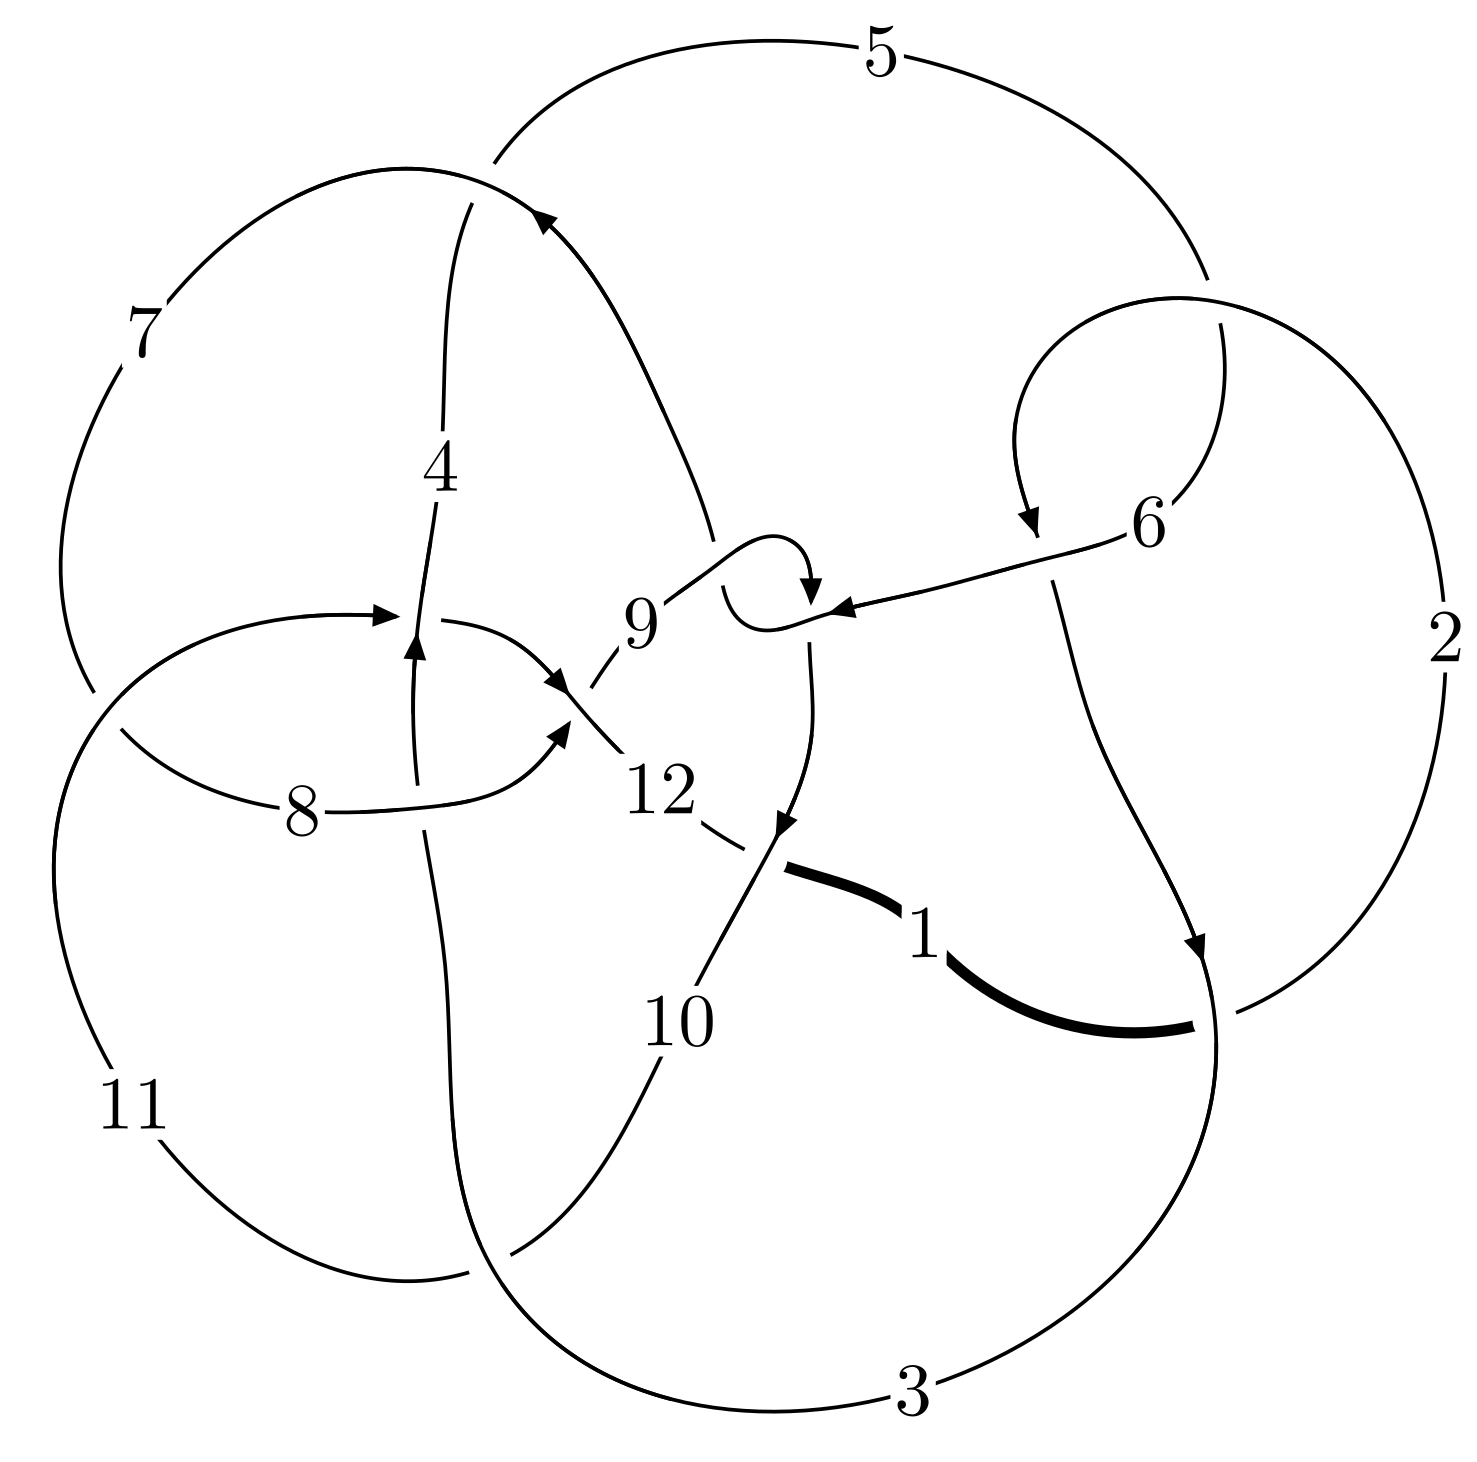
\includegraphics[width=112pt]{../../../GIT/diagram.site/Diagrams/png/2627_12n_0538.png}\\
\ \ \ A knot diagram\footnotemark}&
\allowdisplaybreaks
\textbf{Linearized knot diagam} \\
\cline{2-2}
 &
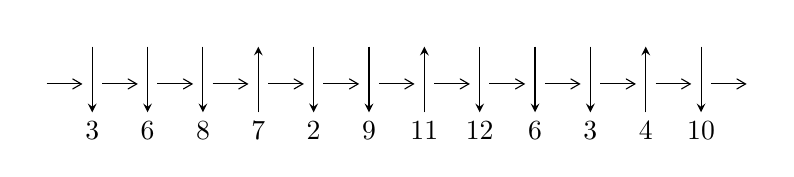
\begin{tikzpicture}[x=20pt, y=17pt]
	% nodes
	\node (C0) at (0, 0) {};
	\node (C1) at (1, 0) {};
	\node (C1U) at (1, +1) {};
	\node (C1D) at (1, -1) {3};

	\node (C2) at (2, 0) {};
	\node (C2U) at (2, +1) {};
	\node (C2D) at (2, -1) {6};

	\node (C3) at (3, 0) {};
	\node (C3U) at (3, +1) {};
	\node (C3D) at (3, -1) {8};

	\node (C4) at (4, 0) {};
	\node (C4U) at (4, +1) {};
	\node (C4D) at (4, -1) {7};

	\node (C5) at (5, 0) {};
	\node (C5U) at (5, +1) {};
	\node (C5D) at (5, -1) {2};

	\node (C6) at (6, 0) {};
	\node (C6U) at (6, +1) {};
	\node (C6D) at (6, -1) {9};

	\node (C7) at (7, 0) {};
	\node (C7U) at (7, +1) {};
	\node (C7D) at (7, -1) {11};

	\node (C8) at (8, 0) {};
	\node (C8U) at (8, +1) {};
	\node (C8D) at (8, -1) {12};

	\node (C9) at (9, 0) {};
	\node (C9U) at (9, +1) {};
	\node (C9D) at (9, -1) {6};

	\node (C10) at (10, 0) {};
	\node (C10U) at (10, +1) {};
	\node (C10D) at (10, -1) {3};

	\node (C11) at (11, 0) {};
	\node (C11U) at (11, +1) {};
	\node (C11D) at (11, -1) {4};

	\node (C12) at (12, 0) {};
	\node (C12U) at (12, +1) {};
	\node (C12D) at (12, -1) {10};
	\node (C13) at (13, 0) {};

	% arrows
	\draw[->,>={angle 60}]
	(C0) edge (C1) (C1) edge (C2) (C2) edge (C3) (C3) edge (C4) (C4) edge (C5) (C5) edge (C6) (C6) edge (C7) (C7) edge (C8) (C8) edge (C9) (C9) edge (C10) (C10) edge (C11) (C11) edge (C12) (C12) edge (C13) ;	\draw[->,>=stealth]
	(C1U) edge (C1D) (C2U) edge (C2D) (C3U) edge (C3D) (C4D) edge (C4U) (C5U) edge (C5D) (C6U) edge (C6D) (C7D) edge (C7U) (C8U) edge (C8D) (C9U) edge (C9D) (C10U) edge (C10D) (C11D) edge (C11U) (C12U) edge (C12D) ;
	\end{tikzpicture} \\
\hhline{~~} \\& 
\textbf{Solving Sequence} \\ \cline{2-2} 
 &
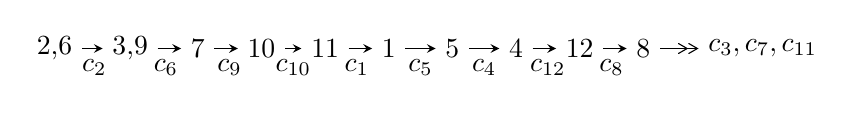
\begin{tikzpicture}[x=23pt, y=7pt]
	% node
	\node (A0) at (-1/8, 0) {2,6};
	\node (A1) at (17/16, 0) {3,9};
	\node (A2) at (17/8, 0) {7};
	\node (A3) at (25/8, 0) {10};
	\node (A4) at (33/8, 0) {11};
	\node (A5) at (41/8, 0) {1};
	\node (A6) at (49/8, 0) {5};
	\node (A7) at (57/8, 0) {4};
	\node (A8) at (65/8, 0) {12};
	\node (A9) at (73/8, 0) {8};
	\node (C1) at (1/2, -1) {$c_{2}$};
	\node (C2) at (13/8, -1) {$c_{6}$};
	\node (C3) at (21/8, -1) {$c_{9}$};
	\node (C4) at (29/8, -1) {$c_{10}$};
	\node (C5) at (37/8, -1) {$c_{1}$};
	\node (C6) at (45/8, -1) {$c_{5}$};
	\node (C7) at (53/8, -1) {$c_{4}$};
	\node (C8) at (61/8, -1) {$c_{12}$};
	\node (C9) at (69/8, -1) {$c_{8}$};
	\node (A10) at (11, 0) {$c_{3},c_{7},c_{11}$};

	% edge
	\draw[->,>=stealth]	
	(A0) edge (A1) (A1) edge (A2) (A2) edge (A3) (A3) edge (A4) (A4) edge (A5) (A5) edge (A6) (A6) edge (A7) (A7) edge (A8) (A8) edge (A9) ;
	\draw[->>,>={angle 60}]	
	(A9) edge (A10);
\end{tikzpicture} \\ 

\end{tabular} \\

\footnotetext{
The image of knot diagram is generated by the software ``\textbf{Draw programme}" developed by Andrew Bartholomew(\url{http://www.layer8.co.uk/maths/draw/index.htm\#Running-draw}), where we modified some parts for our purpose(\url{https://github.com/CATsTAILs/LinksPainter}).
}\phantom \\ \newline 
\centering \textbf{Ideals for irreducible components\footnotemark of $X_{\text{par}}$} 
 
\begin{align*}
I^u_{1}&=\langle 
b- u,\;-1.88153\times10^{15} u^{21}-8.14124\times10^{14} u^{20}+\cdots+7.04162\times10^{15} a-1.77167\times10^{16},\\
\phantom{I^u_{1}}&\phantom{= \langle  }u^{22}+u^{21}+\cdots- u-1\rangle \\
I^u_{2}&=\langle 
3.24728\times10^{55} u^{29}+4.53015\times10^{55} u^{28}+\cdots+1.62069\times10^{57} b+2.03912\times10^{58},\\
\phantom{I^u_{2}}&\phantom{= \langle  }-4.46743\times10^{57} u^{29}-5.44501\times10^{57} u^{28}+\cdots+9.44863\times10^{59} a-4.18593\times10^{60},\\
\phantom{I^u_{2}}&\phantom{= \langle  }u^{30}+2 u^{29}+\cdots+4496 u+583\rangle \\
I^u_{3}&=\langle 
b+u,\;-2 u^{10}-10 u^9-13 u^8+10 u^7+31 u^6+4 u^5-27 u^4-5 u^3+17 u^2+a+5 u-4,\\
\phantom{I^u_{3}}&\phantom{= \langle  }u^{11}+4 u^{10}+2 u^9-9 u^8-8 u^7+9 u^6+9 u^5-7 u^4-6 u^3+3 u^2+2 u-1\rangle \\
I^u_{4}&=\langle 
b+1,\;u^2+a- u,\;u^3- u-1\rangle \\
I^u_{5}&=\langle 
a^2+b+1,\;a^3+a^2+2 a+1,\;u-1\rangle \\
I^u_{6}&=\langle 
b+1,\;a^3+a^2+2 a+1,\;u-1\rangle \\
\\
\end{align*}
\raggedright * 6 irreducible components of $\dim_{\mathbb{C}}=0$, with total 72 representations.\\
\footnotetext{All coefficients of polynomials are rational numbers. But the coefficients are sometimes approximated in decimal forms when there is not enough margin.}
\newpage
\renewcommand{\arraystretch}{1}
\centering \section*{I. $I^u_{1}= \langle b- u,\;-1.88\times10^{15} u^{21}-8.14\times10^{14} u^{20}+\cdots+7.04\times10^{15} a-1.77\times10^{16},\;u^{22}+u^{21}+\cdots- u-1 \rangle$}
\flushleft \textbf{(i) Arc colorings}\\
\begin{tabular}{m{7pt} m{180pt} m{7pt} m{180pt} }
\flushright $a_{2}=$&$\begin{pmatrix}1\\0\end{pmatrix}$ \\
\flushright $a_{6}=$&$\begin{pmatrix}0\\u\end{pmatrix}$ \\
\flushright $a_{3}=$&$\begin{pmatrix}1\\u^2\end{pmatrix}$ \\
\flushright $a_{9}=$&$\begin{pmatrix}0.267202 u^{21}+0.115616 u^{20}+\cdots+5.41231 u+2.51601\\u\end{pmatrix}$ \\
\flushright $a_{7}=$&$\begin{pmatrix}0.617336 u^{21}+0.765365 u^{20}+\cdots-1.29850 u+1.66021\\0.155989 u^{21}+0.149710 u^{20}+\cdots+0.884384 u+0.151586\end{pmatrix}$ \\
\flushright $a_{10}=$&$\begin{pmatrix}0.267202 u^{21}+0.115616 u^{20}+\cdots+5.41231 u+2.51601\\-0.155989 u^{21}-0.149710 u^{20}+\cdots+1.11562 u-0.151586\end{pmatrix}$ \\
\flushright $a_{11}=$&$\begin{pmatrix}0.267202 u^{21}+0.115616 u^{20}+\cdots+4.41231 u+2.51601\\-0.155989 u^{21}-0.149710 u^{20}+\cdots+1.11562 u-0.151586\end{pmatrix}$ \\
\flushright $a_{1}=$&$\begin{pmatrix}- u^2+1\\- u^4\end{pmatrix}$ \\
\flushright $a_{5}=$&$\begin{pmatrix}u\\u\end{pmatrix}$ \\
\flushright $a_{4}=$&$\begin{pmatrix}-0.322075 u^{21}-0.212786 u^{20}+\cdots-6.89909 u-3.09806\\-0.193421 u^{21}-0.0467415 u^{20}+\cdots-0.323268 u-0.397732\end{pmatrix}$ \\
\flushright $a_{12}=$&$\begin{pmatrix}0.305894 u^{21}+0.558047 u^{20}+\cdots-0.813238 u+1.19414\\-0.124057 u^{21}-0.268999 u^{20}+\cdots+0.865623 u+0.408142\end{pmatrix}$ \\
\flushright $a_{8}=$&$\begin{pmatrix}0.536796 u^{21}+0.450130 u^{20}+\cdots+6.96025 u+3.15781\\-0.105547 u^{21}-0.0829132 u^{20}+\cdots+1.39238 u+0.00872824\end{pmatrix}$\\&\end{tabular}
\flushleft \textbf{(ii) Obstruction class $= -1$}\\~\\
\flushleft \textbf{(iii) Cusp Shapes $= \frac{2868088365347525}{4694410161939152} u^{21}-\frac{18112778300119}{586801270242394} u^{20}+\cdots-\frac{981896352987059}{586801270242394} u-\frac{17835381551211165}{4694410161939152}$}\\~\\
\newpage\renewcommand{\arraystretch}{1}
\flushleft \textbf{(iv) u-Polynomials at the component}\newline \\
\begin{tabular}{m{50pt}|m{274pt}}
Crossings & \hspace{64pt}u-Polynomials at each crossing \\
\hline $$\begin{aligned}c_{1}\end{aligned}$$&$\begin{aligned}
&u^{22}+33 u^{21}+\cdots-15 u+1
\end{aligned}$\\
\hline $$\begin{aligned}c_{2},c_{5},c_{10}\end{aligned}$$&$\begin{aligned}
&u^{22}+u^{21}+\cdots- u-1
\end{aligned}$\\
\hline $$\begin{aligned}c_{3},c_{8}\end{aligned}$$&$\begin{aligned}
&u^{22}+u^{21}+\cdots+5 u+1
\end{aligned}$\\
\hline $$\begin{aligned}c_{4}\end{aligned}$$&$\begin{aligned}
&u^{22}+2 u^{21}+\cdots-126 u+103
\end{aligned}$\\
\hline $$\begin{aligned}c_{6},c_{9}\end{aligned}$$&$\begin{aligned}
&u^{22}-10 u^{21}+\cdots-80 u+16
\end{aligned}$\\
\hline $$\begin{aligned}c_{7}\end{aligned}$$&$\begin{aligned}
&u^{22}+u^{21}+\cdots+36 u+8
\end{aligned}$\\
\hline $$\begin{aligned}c_{11}\end{aligned}$$&$\begin{aligned}
&u^{22}-13 u^{21}+\cdots+2 u+4
\end{aligned}$\\
\hline $$\begin{aligned}c_{12}\end{aligned}$$&$\begin{aligned}
&u^{22}+4 u^{21}+\cdots-281 u-83
\end{aligned}$\\
\hline
\end{tabular}\\~\\
\newpage\renewcommand{\arraystretch}{1}
\flushleft \textbf{(v) Riley Polynomials at the component}\newline \\
\begin{tabular}{m{50pt}|m{274pt}}
Crossings & \hspace{64pt}Riley Polynomials at each crossing \\
\hline $$\begin{aligned}c_{1}\end{aligned}$$&$\begin{aligned}
&y^{22}-113 y^{21}+\cdots+107 y+1
\end{aligned}$\\
\hline $$\begin{aligned}c_{2},c_{5},c_{10}\end{aligned}$$&$\begin{aligned}
&y^{22}-33 y^{21}+\cdots+15 y+1
\end{aligned}$\\
\hline $$\begin{aligned}c_{3},c_{8}\end{aligned}$$&$\begin{aligned}
&y^{22}-9 y^{21}+\cdots-25 y+1
\end{aligned}$\\
\hline $$\begin{aligned}c_{4}\end{aligned}$$&$\begin{aligned}
&y^{22}+24 y^{21}+\cdots+134916 y+10609
\end{aligned}$\\
\hline $$\begin{aligned}c_{6},c_{9}\end{aligned}$$&$\begin{aligned}
&y^{22}+6 y^{21}+\cdots-672 y+256
\end{aligned}$\\
\hline $$\begin{aligned}c_{7}\end{aligned}$$&$\begin{aligned}
&y^{22}+13 y^{21}+\cdots+368 y+64
\end{aligned}$\\
\hline $$\begin{aligned}c_{11}\end{aligned}$$&$\begin{aligned}
&y^{22}- y^{21}+\cdots-460 y+16
\end{aligned}$\\
\hline $$\begin{aligned}c_{12}\end{aligned}$$&$\begin{aligned}
&y^{22}-60 y^{21}+\cdots-67175 y+6889
\end{aligned}$\\
\hline
\end{tabular}\\~\\
\newpage\flushleft \textbf{(vi) Complex Volumes and Cusp Shapes}
$$\begin{array}{c|c|c}  
\text{Solutions to }I^u_{1}& \I (\text{vol} + \sqrt{-1}CS) & \text{Cusp shape}\\
 \hline 
\begin{aligned}
u &= -0.748970 + 0.444444 I \\
a &= -0.19228 + 1.51718 I \\
b &= -0.748970 + 0.444444 I\end{aligned}
 & \phantom{-}0.13615 - 1.92714 I & -10.34642 + 1.92836 I \\ \hline\begin{aligned}
u &= -0.748970 - 0.444444 I \\
a &= -0.19228 - 1.51718 I \\
b &= -0.748970 - 0.444444 I\end{aligned}
 & \phantom{-}0.13615 + 1.92714 I & -10.34642 - 1.92836 I \\ \hline\begin{aligned}
u &= -0.130611 + 0.725732 I \\
a &= -1.39284 - 0.49810 I \\
b &= -0.130611 + 0.725732 I\end{aligned}
 & -0.18292 + 6.65611 I & -5.95007 - 7.18766 I \\ \hline\begin{aligned}
u &= -0.130611 - 0.725732 I \\
a &= -1.39284 + 0.49810 I \\
b &= -0.130611 - 0.725732 I\end{aligned}
 & -0.18292 - 6.65611 I & -5.95007 + 7.18766 I \\ \hline\begin{aligned}
u &= \phantom{-}0.401084 + 0.542056 I \\
a &= \phantom{-}1.24737 + 1.06824 I \\
b &= \phantom{-}0.401084 + 0.542056 I\end{aligned}
 & \phantom{-}3.54902 + 1.72435 I & \phantom{-}1.79964 - 0.73697 I \\ \hline\begin{aligned}
u &= \phantom{-}0.401084 - 0.542056 I \\
a &= \phantom{-}1.24737 - 1.06824 I \\
b &= \phantom{-}0.401084 - 0.542056 I\end{aligned}
 & \phantom{-}3.54902 - 1.72435 I & \phantom{-}1.79964 + 0.73697 I \\ \hline\begin{aligned}
u &= -1.33424\phantom{ +0.000000I} \\
a &= -0.431084\phantom{ +0.000000I} \\
b &= -1.33424\phantom{ +0.000000I}\end{aligned}
 & -2.34301\phantom{ +0.000000I} & \phantom{-}2.73470\phantom{ +0.000000I} \\ \hline\begin{aligned}
u &= -0.056775 + 0.629497 I \\
a &= \phantom{-}0.785309 - 1.011460 I \\
b &= -0.056775 + 0.629497 I\end{aligned}
 & -1.31504 + 2.14729 I & -8.96814 - 3.55690 I \\ \hline\begin{aligned}
u &= -0.056775 - 0.629497 I \\
a &= \phantom{-}0.785309 + 1.011460 I \\
b &= -0.056775 - 0.629497 I\end{aligned}
 & -1.31504 - 2.14729 I & -8.96814 + 3.55690 I \\ \hline\begin{aligned}
u &= -0.287480 + 0.350556 I \\
a &= \phantom{-}1.135910 + 0.180293 I \\
b &= -0.287480 + 0.350556 I\end{aligned}
 & -0.788001 + 1.021190 I & -5.92604 - 5.41331 I\\
 \hline 
 \end{array}$$\newpage$$\begin{array}{c|c|c}  
\text{Solutions to }I^u_{1}& \I (\text{vol} + \sqrt{-1}CS) & \text{Cusp shape}\\
 \hline 
\begin{aligned}
u &= -0.287480 - 0.350556 I \\
a &= \phantom{-}1.135910 - 0.180293 I \\
b &= -0.287480 - 0.350556 I\end{aligned}
 & -0.788001 - 1.021190 I & -5.92604 + 5.41331 I \\ \hline\begin{aligned}
u &= \phantom{-}0.181344 + 0.303051 I \\
a &= \phantom{-}1.69533 + 2.92707 I \\
b &= \phantom{-}0.181344 + 0.303051 I\end{aligned}
 & \phantom{-}0.04653 + 2.94961 I & -5.40179 + 1.97738 I \\ \hline\begin{aligned}
u &= \phantom{-}0.181344 - 0.303051 I \\
a &= \phantom{-}1.69533 - 2.92707 I \\
b &= \phantom{-}0.181344 - 0.303051 I\end{aligned}
 & \phantom{-}0.04653 - 2.94961 I & -5.40179 - 1.97738 I \\ \hline\begin{aligned}
u &= \phantom{-}1.76598\phantom{ +0.000000I} \\
a &= \phantom{-}0.362139\phantom{ +0.000000I} \\
b &= \phantom{-}1.76598\phantom{ +0.000000I}\end{aligned}
 & -9.32648\phantom{ +0.000000I} & -9.85720\phantom{ +0.000000I} \\ \hline\begin{aligned}
u &= \phantom{-}1.88020 + 0.16813 I \\
a &= \phantom{-}0.593976 + 0.598808 I \\
b &= \phantom{-}1.88020 + 0.16813 I\end{aligned}
 & -13.59180 - 1.67864 I & -10.72705 - 0.48573 I \\ \hline\begin{aligned}
u &= \phantom{-}1.88020 - 0.16813 I \\
a &= \phantom{-}0.593976 - 0.598808 I \\
b &= \phantom{-}1.88020 - 0.16813 I\end{aligned}
 & -13.59180 + 1.67864 I & -10.72705 + 0.48573 I \\ \hline\begin{aligned}
u &= -1.95173 + 0.18984 I \\
a &= -0.792024 + 0.526959 I \\
b &= -1.95173 + 0.18984 I\end{aligned}
 & -15.4135 - 5.6943 I & -10.05870 + 3.46761 I \\ \hline\begin{aligned}
u &= -1.95173 - 0.18984 I \\
a &= -0.792024 - 0.526959 I \\
b &= -1.95173 - 0.18984 I\end{aligned}
 & -15.4135 + 5.6943 I & -10.05870 - 3.46761 I \\ \hline\begin{aligned}
u &= \phantom{-}1.97172 + 0.33031 I \\
a &= \phantom{-}0.661105 + 0.393921 I \\
b &= \phantom{-}1.97172 + 0.33031 I\end{aligned}
 & -14.3712 - 6.4475 I & -12.31821 + 5.34631 I \\ \hline\begin{aligned}
u &= \phantom{-}1.97172 - 0.33031 I \\
a &= \phantom{-}0.661105 - 0.393921 I \\
b &= \phantom{-}1.97172 - 0.33031 I\end{aligned}
 & -14.3712 + 6.4475 I & -12.31821 - 5.34631 I\\
 \hline 
 \end{array}$$\newpage$$\begin{array}{c|c|c}  
\text{Solutions to }I^u_{1}& \I (\text{vol} + \sqrt{-1}CS) & \text{Cusp shape}\\
 \hline 
\begin{aligned}
u &= -1.97465 + 0.36872 I \\
a &= -0.707383 + 0.533233 I \\
b &= -1.97465 + 0.36872 I\end{aligned}
 & -14.7419 + 15.2513 I & -9.04193 - 6.95312 I \\ \hline\begin{aligned}
u &= -1.97465 - 0.36872 I \\
a &= -0.707383 - 0.533233 I \\
b &= -1.97465 - 0.36872 I\end{aligned}
 & -14.7419 - 15.2513 I & -9.04193 + 6.95312 I\\
 \hline 
 \end{array}$$\newpage\newpage\renewcommand{\arraystretch}{1}
\centering \section*{II. $I^u_{2}= \langle 3.25\times10^{55} u^{29}+4.53\times10^{55} u^{28}+\cdots+1.62\times10^{57} b+2.04\times10^{58},\;-4.47\times10^{57} u^{29}-5.45\times10^{57} u^{28}+\cdots+9.45\times10^{59} a-4.19\times10^{60},\;u^{30}+2 u^{29}+\cdots+4496 u+583 \rangle$}
\flushleft \textbf{(i) Arc colorings}\\
\begin{tabular}{m{7pt} m{180pt} m{7pt} m{180pt} }
\flushright $a_{2}=$&$\begin{pmatrix}1\\0\end{pmatrix}$ \\
\flushright $a_{6}=$&$\begin{pmatrix}0\\u\end{pmatrix}$ \\
\flushright $a_{3}=$&$\begin{pmatrix}1\\u^2\end{pmatrix}$ \\
\flushright $a_{9}=$&$\begin{pmatrix}0.00472813 u^{29}+0.00576275 u^{28}+\cdots+27.0557 u+4.43020\\-0.0200364 u^{29}-0.0279520 u^{28}+\cdots-67.4156 u-12.5818\end{pmatrix}$ \\
\flushright $a_{7}=$&$\begin{pmatrix}0.00410451 u^{29}+0.0121031 u^{28}+\cdots+6.61203 u+1.98039\\0.00745135 u^{29}+0.0160502 u^{28}+\cdots+0.792830 u+0.0832540\end{pmatrix}$ \\
\flushright $a_{10}=$&$\begin{pmatrix}0.00472813 u^{29}+0.00576275 u^{28}+\cdots+27.0557 u+4.43020\\-0.0171807 u^{29}-0.0229105 u^{28}+\cdots-53.5661 u-10.4285\end{pmatrix}$ \\
\flushright $a_{11}=$&$\begin{pmatrix}0.0247645 u^{29}+0.0337147 u^{28}+\cdots+94.4714 u+17.0120\\-0.00141883 u^{29}-0.00143599 u^{28}+\cdots-10.7523 u-3.36205\end{pmatrix}$ \\
\flushright $a_{1}=$&$\begin{pmatrix}- u^2+1\\- u^4\end{pmatrix}$ \\
\flushright $a_{5}=$&$\begin{pmatrix}u\\u\end{pmatrix}$ \\
\flushright $a_{4}=$&$\begin{pmatrix}-0.00504933 u^{29}-0.00945349 u^{28}+\cdots-40.1713 u-6.41129\\0.00262810 u^{29}+0.00887618 u^{28}+\cdots-27.9565 u-3.77015\end{pmatrix}$ \\
\flushright $a_{12}=$&$\begin{pmatrix}0.00260386 u^{29}+0.00679584 u^{28}+\cdots-7.78421 u+2.10200\\-0.0131077 u^{29}-0.00690705 u^{28}+\cdots-102.987 u-16.3636\end{pmatrix}$ \\
\flushright $a_{8}=$&$\begin{pmatrix}0.00606568 u^{29}+0.0116476 u^{28}+\cdots+9.85622 u-0.550040\\0.00608037 u^{29}+0.0164677 u^{28}+\cdots-17.2937 u-1.45033\end{pmatrix}$\\&\end{tabular}
\flushleft \textbf{(ii) Obstruction class $= -1$}\\~\\
\flushleft \textbf{(iii) Cusp Shapes $= 0.261146 u^{29}+0.287455 u^{28}+\cdots+1402.90 u+219.809$}\\~\\
\newpage\renewcommand{\arraystretch}{1}
\flushleft \textbf{(iv) u-Polynomials at the component}\newline \\
\begin{tabular}{m{50pt}|m{274pt}}
Crossings & \hspace{64pt}u-Polynomials at each crossing \\
\hline $$\begin{aligned}c_{1}\end{aligned}$$&$\begin{aligned}
&u^{30}+46 u^{29}+\cdots+11608936 u+339889
\end{aligned}$\\
\hline $$\begin{aligned}c_{2},c_{5},c_{10}\end{aligned}$$&$\begin{aligned}
&u^{30}+2 u^{29}+\cdots+4496 u+583
\end{aligned}$\\
\hline $$\begin{aligned}c_{3},c_{8}\end{aligned}$$&$\begin{aligned}
&u^{30}+u^{29}+\cdots+58 u-11
\end{aligned}$\\
\hline $$\begin{aligned}c_{4}\end{aligned}$$&$\begin{aligned}
&u^{30}+8 u^{29}+\cdots+2447 u+271
\end{aligned}$\\
\hline $$\begin{aligned}c_{6},c_{9}\end{aligned}$$&$\begin{aligned}
&(u^{15}+7 u^{14}+\cdots+4 u+1)^{2}
\end{aligned}$\\
\hline $$\begin{aligned}c_{7}\end{aligned}$$&$\begin{aligned}
&u^{30}+3 u^{29}+\cdots+356 u+88
\end{aligned}$\\
\hline $$\begin{aligned}c_{11}\end{aligned}$$&$\begin{aligned}
&(u^{15}+8 u^{14}+\cdots+5 u+1)^{2}
\end{aligned}$\\
\hline $$\begin{aligned}c_{12}\end{aligned}$$&$\begin{aligned}
&u^{30}+2 u^{29}+\cdots+197368 u-32296
\end{aligned}$\\
\hline
\end{tabular}\\~\\
\newpage\renewcommand{\arraystretch}{1}
\flushleft \textbf{(v) Riley Polynomials at the component}\newline \\
\begin{tabular}{m{50pt}|m{274pt}}
Crossings & \hspace{64pt}Riley Polynomials at each crossing \\
\hline $$\begin{aligned}c_{1}\end{aligned}$$&$\begin{aligned}
&y^{30}-50 y^{29}+\cdots-48946220611468 y+115524532321
\end{aligned}$\\
\hline $$\begin{aligned}c_{2},c_{5},c_{10}\end{aligned}$$&$\begin{aligned}
&y^{30}-46 y^{29}+\cdots-11608936 y+339889
\end{aligned}$\\
\hline $$\begin{aligned}c_{3},c_{8}\end{aligned}$$&$\begin{aligned}
&y^{30}-3 y^{29}+\cdots-3056 y+121
\end{aligned}$\\
\hline $$\begin{aligned}c_{4}\end{aligned}$$&$\begin{aligned}
&y^{30}+64 y^{29}+\cdots-1263195 y+73441
\end{aligned}$\\
\hline $$\begin{aligned}c_{6},c_{9}\end{aligned}$$&$\begin{aligned}
&(y^{15}-3 y^{14}+\cdots+36 y-1)^{2}
\end{aligned}$\\
\hline $$\begin{aligned}c_{7}\end{aligned}$$&$\begin{aligned}
&y^{30}+17 y^{29}+\cdots+280176 y+7744
\end{aligned}$\\
\hline $$\begin{aligned}c_{11}\end{aligned}$$&$\begin{aligned}
&(y^{15}+28 y^{13}+\cdots-9 y-1)^{2}
\end{aligned}$\\
\hline $$\begin{aligned}c_{12}\end{aligned}$$&$\begin{aligned}
&y^{30}-22 y^{29}+\cdots-9540868384 y+1043031616
\end{aligned}$\\
\hline
\end{tabular}\\~\\
\newpage\flushleft \textbf{(vi) Complex Volumes and Cusp Shapes}
$$\begin{array}{c|c|c}  
\text{Solutions to }I^u_{2}& \I (\text{vol} + \sqrt{-1}CS) & \text{Cusp shape}\\
 \hline 
\begin{aligned}
u &= \phantom{-}0.733366 + 0.760399 I \\
a &= -0.932743 + 0.643875 I \\
b &= -1.086660 + 0.495175 I\end{aligned}
 & -3.92076 - 0.11084 I & -19.2470 + 2.6115 I \\ \hline\begin{aligned}
u &= \phantom{-}0.733366 - 0.760399 I \\
a &= -0.932743 - 0.643875 I \\
b &= -1.086660 - 0.495175 I\end{aligned}
 & -3.92076 + 0.11084 I & -19.2470 - 2.6115 I \\ \hline\begin{aligned}
u &= \phantom{-}1.102460 + 0.135538 I \\
a &= \phantom{-}0.850106 - 0.383862 I \\
b &= \phantom{-}1.20887 - 1.10475 I\end{aligned}
 & -4.14672 + 8.45942 I & -10.28669 - 6.66978 I \\ \hline\begin{aligned}
u &= \phantom{-}1.102460 - 0.135538 I \\
a &= \phantom{-}0.850106 + 0.383862 I \\
b &= \phantom{-}1.20887 + 1.10475 I\end{aligned}
 & -4.14672 - 8.45942 I & -10.28669 + 6.66978 I \\ \hline\begin{aligned}
u &= -0.873450 + 0.022311 I \\
a &= -0.450314 - 0.183725 I \\
b &= -1.86355 + 1.25575 I\end{aligned}
 & -2.83938 + 0.15495 I & -69.8860 - 16.0941 I \\ \hline\begin{aligned}
u &= -0.873450 - 0.022311 I \\
a &= -0.450314 + 0.183725 I \\
b &= -1.86355 - 1.25575 I\end{aligned}
 & -2.83938 - 0.15495 I & -69.8860 + 16.0941 I \\ \hline\begin{aligned}
u &= -0.965004 + 0.592094 I \\
a &= \phantom{-}0.798906 + 0.014589 I \\
b &= \phantom{-}1.027040 + 0.648501 I\end{aligned}
 & -2.16274 + 2.22327 I & -10.93751 - 4.89170 I \\ \hline\begin{aligned}
u &= -0.965004 - 0.592094 I \\
a &= \phantom{-}0.798906 - 0.014589 I \\
b &= \phantom{-}1.027040 - 0.648501 I\end{aligned}
 & -2.16274 - 2.22327 I & -10.93751 + 4.89170 I \\ \hline\begin{aligned}
u &= \phantom{-}1.133110 + 0.242313 I \\
a &= -0.356690 - 1.137480 I \\
b &= -0.340336 - 0.281341 I\end{aligned}
 & \phantom{-}1.41649 - 4.96313 I & -5.21468 + 7.56800 I \\ \hline\begin{aligned}
u &= \phantom{-}1.133110 - 0.242313 I \\
a &= -0.356690 + 1.137480 I \\
b &= -0.340336 + 0.281341 I\end{aligned}
 & \phantom{-}1.41649 + 4.96313 I & -5.21468 - 7.56800 I\\
 \hline 
 \end{array}$$\newpage$$\begin{array}{c|c|c}  
\text{Solutions to }I^u_{2}& \I (\text{vol} + \sqrt{-1}CS) & \text{Cusp shape}\\
 \hline 
\begin{aligned}
u &= -1.086660 + 0.495175 I \\
a &= \phantom{-}0.812020 + 0.588181 I \\
b &= \phantom{-}0.733366 + 0.760399 I\end{aligned}
 & -3.92076 - 0.11084 I & -19.2470 + 2.6115 I \\ \hline\begin{aligned}
u &= -1.086660 - 0.495175 I \\
a &= \phantom{-}0.812020 - 0.588181 I \\
b &= \phantom{-}0.733366 - 0.760399 I\end{aligned}
 & -3.92076 + 0.11084 I & -19.2470 - 2.6115 I \\ \hline\begin{aligned}
u &= \phantom{-}1.027040 + 0.648501 I \\
a &= -0.340958 + 0.662159 I \\
b &= -0.965004 + 0.592094 I\end{aligned}
 & -2.16274 + 2.22327 I & -10.93751 - 4.89170 I \\ \hline\begin{aligned}
u &= \phantom{-}1.027040 - 0.648501 I \\
a &= -0.340958 - 0.662159 I \\
b &= -0.965004 - 0.592094 I\end{aligned}
 & -2.16274 - 2.22327 I & -10.93751 + 4.89170 I \\ \hline\begin{aligned}
u &= -1.24424\phantom{ +0.000000I} \\
a &= \phantom{-}0.162086\phantom{ +0.000000I} \\
b &= -0.214799\phantom{ +0.000000I}\end{aligned}
 & -2.25644\phantom{ +0.000000I} & \phantom{-}3.80230\phantom{ +0.000000I} \\ \hline\begin{aligned}
u &= -0.340336 + 0.281341 I \\
a &= \phantom{-}2.20884 - 2.21512 I \\
b &= \phantom{-}1.133110 - 0.242313 I\end{aligned}
 & \phantom{-}1.41649 + 4.96313 I & -5.21468 - 7.56800 I \\ \hline\begin{aligned}
u &= -0.340336 - 0.281341 I \\
a &= \phantom{-}2.20884 + 2.21512 I \\
b &= \phantom{-}1.133110 + 0.242313 I\end{aligned}
 & \phantom{-}1.41649 - 4.96313 I & -5.21468 + 7.56800 I \\ \hline\begin{aligned}
u &= \phantom{-}1.20887 + 1.10475 I \\
a &= \phantom{-}0.572773 - 0.268684 I \\
b &= \phantom{-}1.102460 - 0.135538 I\end{aligned}
 & -4.14672 - 8.45942 I & -6.00000 + 6.66978 I \\ \hline\begin{aligned}
u &= \phantom{-}1.20887 - 1.10475 I \\
a &= \phantom{-}0.572773 + 0.268684 I \\
b &= \phantom{-}1.102460 + 0.135538 I\end{aligned}
 & -4.14672 + 8.45942 I & -6.00000 - 6.66978 I \\ \hline\begin{aligned}
u &= -0.214799\phantom{ +0.000000I} \\
a &= \phantom{-}0.938895\phantom{ +0.000000I} \\
b &= -1.24424\phantom{ +0.000000I}\end{aligned}
 & -2.25644\phantom{ +0.000000I} & \phantom{-}3.80230\phantom{ +0.000000I}\\
 \hline 
 \end{array}$$\newpage$$\begin{array}{c|c|c}  
\text{Solutions to }I^u_{2}& \I (\text{vol} + \sqrt{-1}CS) & \text{Cusp shape}\\
 \hline 
\begin{aligned}
u &= \phantom{-}1.81586 + 0.25309 I \\
a &= -0.879383 - 0.431389 I \\
b &= -2.13925 - 0.18775 I\end{aligned}
 & -14.0337 - 3.5387 I & \phantom{-0.000000 } 0 \\ \hline\begin{aligned}
u &= \phantom{-}1.81586 - 0.25309 I \\
a &= -0.879383 + 0.431389 I \\
b &= -2.13925 + 0.18775 I\end{aligned}
 & -14.0337 + 3.5387 I & \phantom{-0.000000 } 0 \\ \hline\begin{aligned}
u &= \phantom{-}1.88905 + 0.21159 I \\
a &= -0.720062 - 0.679808 I \\
b &= -1.91198 - 0.46830 I\end{aligned}
 & -12.66340 - 6.19285 I & \phantom{-0.000000 } 0 \\ \hline\begin{aligned}
u &= \phantom{-}1.88905 - 0.21159 I \\
a &= -0.720062 + 0.679808 I \\
b &= -1.91198 + 0.46830 I\end{aligned}
 & -12.66340 + 6.19285 I & \phantom{-0.000000 } 0 \\ \hline\begin{aligned}
u &= -1.91198 + 0.46830 I \\
a &= \phantom{-}0.773799 - 0.561815 I \\
b &= \phantom{-}1.88905 - 0.21159 I\end{aligned}
 & -12.66340 + 6.19285 I & \phantom{-0.000000 } 0 \\ \hline\begin{aligned}
u &= -1.91198 - 0.46830 I \\
a &= \phantom{-}0.773799 + 0.561815 I \\
b &= \phantom{-}1.88905 + 0.21159 I\end{aligned}
 & -12.66340 - 6.19285 I & \phantom{-0.000000 } 0 \\ \hline\begin{aligned}
u &= -2.13925 + 0.18775 I \\
a &= \phantom{-}0.731046 - 0.406052 I \\
b &= \phantom{-}1.81586 - 0.25309 I\end{aligned}
 & -14.0337 + 3.5387 I & \phantom{-0.000000 } 0 \\ \hline\begin{aligned}
u &= -2.13925 - 0.18775 I \\
a &= \phantom{-}0.731046 + 0.406052 I \\
b &= \phantom{-}1.81586 + 0.25309 I\end{aligned}
 & -14.0337 - 3.5387 I & \phantom{-0.000000 } 0 \\ \hline\begin{aligned}
u &= -1.86355 + 1.25575 I \\
a &= -0.109258 - 0.154344 I \\
b &= -0.873450 + 0.022311 I\end{aligned}
 & -2.83938 + 0.15495 I & \phantom{-0.000000 } 0 \\ \hline\begin{aligned}
u &= -1.86355 - 1.25575 I \\
a &= -0.109258 + 0.154344 I \\
b &= -0.873450 - 0.022311 I\end{aligned}
 & -2.83938 - 0.15495 I & \phantom{-0.000000 } 0\\
 \hline 
 \end{array}$$\newpage\newpage\renewcommand{\arraystretch}{1}
\centering \section*{III. $I^u_{3}= \langle b+u,\;-2 u^{10}-10 u^9+\cdots+a-4,\;u^{11}+4 u^{10}+\cdots+2 u-1 \rangle$}
\flushleft \textbf{(i) Arc colorings}\\
\begin{tabular}{m{7pt} m{180pt} m{7pt} m{180pt} }
\flushright $a_{2}=$&$\begin{pmatrix}1\\0\end{pmatrix}$ \\
\flushright $a_{6}=$&$\begin{pmatrix}0\\u\end{pmatrix}$ \\
\flushright $a_{3}=$&$\begin{pmatrix}1\\u^2\end{pmatrix}$ \\
\flushright $a_{9}=$&$\begin{pmatrix}2 u^{10}+10 u^9+\cdots-5 u+4\\- u\end{pmatrix}$ \\
\flushright $a_{7}=$&$\begin{pmatrix}4 u^{10}+17 u^9+\cdots+u+6\\u^{10}+4 u^9+3 u^8-6 u^7-9 u^6+u^5+9 u^4+u^3-6 u^2- u+2\end{pmatrix}$ \\
\flushright $a_{10}=$&$\begin{pmatrix}2 u^{10}+10 u^9+\cdots-5 u+4\\u^{10}+4 u^9+3 u^8-6 u^7-9 u^6+u^5+9 u^4+u^3-6 u^2-3 u+2\end{pmatrix}$ \\
\flushright $a_{11}=$&$\begin{pmatrix}2 u^{10}+10 u^9+\cdots-4 u+4\\u^{10}+4 u^9+3 u^8-6 u^7-9 u^6+u^5+9 u^4+2 u^3-6 u^2-3 u+2\end{pmatrix}$ \\
\flushright $a_{1}=$&$\begin{pmatrix}- u^2+1\\- u^4\end{pmatrix}$ \\
\flushright $a_{5}=$&$\begin{pmatrix}u\\u\end{pmatrix}$ \\
\flushright $a_{4}=$&$\begin{pmatrix}-4 u^{10}-18 u^9+\cdots+3 u-5\\-2 u^9-7 u^8- u^7+16 u^6+6 u^5-15 u^4-4 u^3+10 u^2+2 u-2\end{pmatrix}$ \\
\flushright $a_{12}=$&$\begin{pmatrix}3 u^{10}+13 u^9+\cdots-2 u+6\\u^{10}+5 u^9+5 u^8-10 u^7-16 u^6+8 u^5+16 u^4-5 u^3-10 u^2+u+2\end{pmatrix}$ \\
\flushright $a_{8}=$&$\begin{pmatrix}6 u^{10}+25 u^9+\cdots-4 u+8\\2 u^{10}+8 u^9+5 u^8-14 u^7-14 u^6+10 u^5+12 u^4-7 u^3-7 u^2+u+1\end{pmatrix}$\\&\end{tabular}
\flushleft \textbf{(ii) Obstruction class $= 1$}\\~\\
\flushleft \textbf{(iii) Cusp Shapes $= -11 u^{10}-54 u^9-64 u^8+66 u^7+156 u^6-8 u^5-139 u^4-6 u^3+92 u^2+14 u-33$}\\~\\
\newpage\renewcommand{\arraystretch}{1}
\flushleft \textbf{(iv) u-Polynomials at the component}\newline \\
\begin{tabular}{m{50pt}|m{274pt}}
Crossings & \hspace{64pt}u-Polynomials at each crossing \\
\hline $$\begin{aligned}c_{1}\end{aligned}$$&$\begin{aligned}
&u^{11}-12 u^{10}+\cdots+10 u-1
\end{aligned}$\\
\hline $$\begin{aligned}c_{2},c_{10}\end{aligned}$$&$\begin{aligned}
&u^{11}+4 u^{10}+2 u^9-9 u^8-8 u^7+9 u^6+9 u^5-7 u^4-6 u^3+3 u^2+2 u-1
\end{aligned}$\\
\hline $$\begin{aligned}c_{3},c_{8}\end{aligned}$$&$\begin{aligned}
&u^{11}- u^9+u^8+3 u^7- u^6- u^5-2 u^4-2 u^3+3 u^2+u-1
\end{aligned}$\\
\hline $$\begin{aligned}c_{4}\end{aligned}$$&$\begin{aligned}
&u^{11}+u^{10}+4 u^9+u^8+7 u^7-4 u^6-3 u^5-7 u^4+5 u^3+u^2-1
\end{aligned}$\\
\hline $$\begin{aligned}c_{5}\end{aligned}$$&$\begin{aligned}
&u^{11}-4 u^{10}+2 u^9+9 u^8-8 u^7-9 u^6+9 u^5+7 u^4-6 u^3-3 u^2+2 u+1
\end{aligned}$\\
\hline $$\begin{aligned}c_{6}\end{aligned}$$&$\begin{aligned}
&u^{11}-4 u^{10}+\cdots+4 u-1
\end{aligned}$\\
\hline $$\begin{aligned}c_{7}\end{aligned}$$&$\begin{aligned}
&u^{11}+u^{10}+\cdots+9 u+1
\end{aligned}$\\
\hline $$\begin{aligned}c_{9}\end{aligned}$$&$\begin{aligned}
&u^{11}+4 u^{10}+\cdots+4 u+1
\end{aligned}$\\
\hline $$\begin{aligned}c_{11}\end{aligned}$$&$\begin{aligned}
&u^{11}-5 u^{10}+13 u^9-20 u^8+20 u^7-13 u^6+7 u^5-5 u^4+3 u^3- u^2-1
\end{aligned}$\\
\hline $$\begin{aligned}c_{12}\end{aligned}$$&$\begin{aligned}
&u^{11}+7 u^{10}+\cdots+7 u+1
\end{aligned}$\\
\hline
\end{tabular}\\~\\
\newpage\renewcommand{\arraystretch}{1}
\flushleft \textbf{(v) Riley Polynomials at the component}\newline \\
\begin{tabular}{m{50pt}|m{274pt}}
Crossings & \hspace{64pt}Riley Polynomials at each crossing \\
\hline $$\begin{aligned}c_{1}\end{aligned}$$&$\begin{aligned}
&y^{11}-24 y^{10}+\cdots+6 y-1
\end{aligned}$\\
\hline $$\begin{aligned}c_{2},c_{5},c_{10}\end{aligned}$$&$\begin{aligned}
&y^{11}-12 y^{10}+\cdots+10 y-1
\end{aligned}$\\
\hline $$\begin{aligned}c_{3},c_{8}\end{aligned}$$&$\begin{aligned}
&y^{11}-2 y^{10}+\cdots+7 y-1
\end{aligned}$\\
\hline $$\begin{aligned}c_{4}\end{aligned}$$&$\begin{aligned}
&y^{11}+7 y^{10}+\cdots+2 y-1
\end{aligned}$\\
\hline $$\begin{aligned}c_{6},c_{9}\end{aligned}$$&$\begin{aligned}
&y^{11}+6 y^{10}+\cdots-6 y-1
\end{aligned}$\\
\hline $$\begin{aligned}c_{7}\end{aligned}$$&$\begin{aligned}
&y^{11}+7 y^{10}+\cdots+59 y-1
\end{aligned}$\\
\hline $$\begin{aligned}c_{11}\end{aligned}$$&$\begin{aligned}
&y^{11}+y^{10}+\cdots-2 y-1
\end{aligned}$\\
\hline $$\begin{aligned}c_{12}\end{aligned}$$&$\begin{aligned}
&y^{11}-17 y^{10}+\cdots-7 y-1
\end{aligned}$\\
\hline
\end{tabular}\\~\\
\newpage\flushleft \textbf{(vi) Complex Volumes and Cusp Shapes}
$$\begin{array}{c|c|c}  
\text{Solutions to }I^u_{3}& \I (\text{vol} + \sqrt{-1}CS) & \text{Cusp shape}\\
 \hline 
\begin{aligned}
u &= -0.783748 + 0.507589 I \\
a &= -0.655301 + 0.652413 I \\
b &= \phantom{-}0.783748 - 0.507589 I\end{aligned}
 & -1.51867 + 8.25174 I & -7.26021 - 7.31178 I \\ \hline\begin{aligned}
u &= -0.783748 - 0.507589 I \\
a &= -0.655301 - 0.652413 I \\
b &= \phantom{-}0.783748 + 0.507589 I\end{aligned}
 & -1.51867 - 8.25174 I & -7.26021 + 7.31178 I \\ \hline\begin{aligned}
u &= \phantom{-}1.09593\phantom{ +0.000000I} \\
a &= -0.532565\phantom{ +0.000000I} \\
b &= -1.09593\phantom{ +0.000000I}\end{aligned}
 & -2.75997\phantom{ +0.000000I} & -16.4390\phantom{ +0.000000I} \\ \hline\begin{aligned}
u &= -1.038820 + 0.472232 I \\
a &= \phantom{-}0.374208 - 1.064480 I \\
b &= \phantom{-}1.038820 - 0.472232 I\end{aligned}
 & \phantom{-}0.22754 + 6.88359 I & -6.74283 - 7.96199 I \\ \hline\begin{aligned}
u &= -1.038820 - 0.472232 I \\
a &= \phantom{-}0.374208 + 1.064480 I \\
b &= \phantom{-}1.038820 + 0.472232 I\end{aligned}
 & \phantom{-}0.22754 - 6.88359 I & -6.74283 + 7.96199 I \\ \hline\begin{aligned}
u &= \phantom{-}0.688260 + 0.474217 I \\
a &= \phantom{-}0.128118 + 0.656640 I \\
b &= -0.688260 - 0.474217 I\end{aligned}
 & -2.33645 - 0.11538 I & -12.41153 + 0.34745 I \\ \hline\begin{aligned}
u &= \phantom{-}0.688260 - 0.474217 I \\
a &= \phantom{-}0.128118 - 0.656640 I \\
b &= -0.688260 + 0.474217 I\end{aligned}
 & -2.33645 + 0.11538 I & -12.41153 - 0.34745 I \\ \hline\begin{aligned}
u &= \phantom{-}0.526465 + 0.148349 I \\
a &= -1.33892 - 1.68823 I \\
b &= -0.526465 - 0.148349 I\end{aligned}
 & -0.17031 - 3.59582 I & -8.70170 + 8.76278 I \\ \hline\begin{aligned}
u &= \phantom{-}0.526465 - 0.148349 I \\
a &= -1.33892 + 1.68823 I \\
b &= -0.526465 + 0.148349 I\end{aligned}
 & -0.17031 + 3.59582 I & -8.70170 - 8.76278 I \\ \hline\begin{aligned}
u &= -1.94012 + 0.28522 I \\
a &= \phantom{-}0.758182 - 0.505152 I \\
b &= \phantom{-}1.94012 - 0.28522 I\end{aligned}
 & -12.91640 + 4.72001 I & -9.66405 - 2.38742 I\\
 \hline 
 \end{array}$$\newpage$$\begin{array}{c|c|c}  
\text{Solutions to }I^u_{3}& \I (\text{vol} + \sqrt{-1}CS) & \text{Cusp shape}\\
 \hline 
\begin{aligned}
u &= -1.94012 - 0.28522 I \\
a &= \phantom{-}0.758182 + 0.505152 I \\
b &= \phantom{-}1.94012 + 0.28522 I\end{aligned}
 & -12.91640 - 4.72001 I & -9.66405 + 2.38742 I\\
 \hline 
 \end{array}$$\newpage\newpage\renewcommand{\arraystretch}{1}
\centering \section*{IV. $I^u_{4}= \langle b+1,\;u^2+a- u,\;u^3- u-1 \rangle$}
\flushleft \textbf{(i) Arc colorings}\\
\begin{tabular}{m{7pt} m{180pt} m{7pt} m{180pt} }
\flushright $a_{2}=$&$\begin{pmatrix}1\\0\end{pmatrix}$ \\
\flushright $a_{6}=$&$\begin{pmatrix}0\\u\end{pmatrix}$ \\
\flushright $a_{3}=$&$\begin{pmatrix}1\\u^2\end{pmatrix}$ \\
\flushright $a_{9}=$&$\begin{pmatrix}- u^2+u\\-1\end{pmatrix}$ \\
\flushright $a_{7}=$&$\begin{pmatrix}u^2-2\\u^2-1\end{pmatrix}$ \\
\flushright $a_{10}=$&$\begin{pmatrix}- u^2+u\\- u^2\end{pmatrix}$ \\
\flushright $a_{11}=$&$\begin{pmatrix}- u^2+u+1\\0\end{pmatrix}$ \\
\flushright $a_{1}=$&$\begin{pmatrix}- u^2+1\\- u^2- u\end{pmatrix}$ \\
\flushright $a_{5}=$&$\begin{pmatrix}u\\u\end{pmatrix}$ \\
\flushright $a_{4}=$&$\begin{pmatrix}1\\u+1\end{pmatrix}$ \\
\flushright $a_{12}=$&$\begin{pmatrix}- u^2+1\\- u^2- u\end{pmatrix}$ \\
\flushright $a_{8}=$&$\begin{pmatrix}0\\u^2-1\end{pmatrix}$\\&\end{tabular}
\flushleft \textbf{(ii) Obstruction class $= 1$}\\~\\
\flushleft \textbf{(iii) Cusp Shapes $= -7 u^2- u-5$}\\~\\
\newpage\renewcommand{\arraystretch}{1}
\flushleft \textbf{(iv) u-Polynomials at the component}\newline \\
\begin{tabular}{m{50pt}|m{274pt}}
Crossings & \hspace{64pt}u-Polynomials at each crossing \\
\hline $$\begin{aligned}c_{1}\end{aligned}$$&$\begin{aligned}
&u^3-2 u^2+u-1
\end{aligned}$\\
\hline $$\begin{aligned}c_{2},c_{4},c_{11}\end{aligned}$$&$\begin{aligned}
&u^3- u-1
\end{aligned}$\\
\hline $$\begin{aligned}c_{3}\end{aligned}$$&$\begin{aligned}
&u^3+u^2-1
\end{aligned}$\\
\hline $$\begin{aligned}c_{5}\end{aligned}$$&$\begin{aligned}
&u^3- u+1
\end{aligned}$\\
\hline $$\begin{aligned}c_{6},c_{8}\end{aligned}$$&$\begin{aligned}
&u^3- u^2+2 u-1
\end{aligned}$\\
\hline $$\begin{aligned}c_{7}\end{aligned}$$&$\begin{aligned}
&u^3+2 u^2+3 u+1
\end{aligned}$\\
\hline $$\begin{aligned}c_{9}\end{aligned}$$&$\begin{aligned}
&u^3+u^2+2 u+1
\end{aligned}$\\
\hline $$\begin{aligned}c_{10}\end{aligned}$$&$\begin{aligned}
&(u-1)^3
\end{aligned}$\\
\hline $$\begin{aligned}c_{12}\end{aligned}$$&$\begin{aligned}
&u^3
\end{aligned}$\\
\hline
\end{tabular}\\~\\
\newpage\renewcommand{\arraystretch}{1}
\flushleft \textbf{(v) Riley Polynomials at the component}\newline \\
\begin{tabular}{m{50pt}|m{274pt}}
Crossings & \hspace{64pt}Riley Polynomials at each crossing \\
\hline $$\begin{aligned}c_{1}\end{aligned}$$&$\begin{aligned}
&y^3-2 y^2-3 y-1
\end{aligned}$\\
\hline $$\begin{aligned}c_{2},c_{4},c_{5}\\c_{11}\end{aligned}$$&$\begin{aligned}
&y^3-2 y^2+y-1
\end{aligned}$\\
\hline $$\begin{aligned}c_{3}\end{aligned}$$&$\begin{aligned}
&y^3- y^2+2 y-1
\end{aligned}$\\
\hline $$\begin{aligned}c_{6},c_{8},c_{9}\end{aligned}$$&$\begin{aligned}
&y^3+3 y^2+2 y-1
\end{aligned}$\\
\hline $$\begin{aligned}c_{7}\end{aligned}$$&$\begin{aligned}
&y^3+2 y^2+5 y-1
\end{aligned}$\\
\hline $$\begin{aligned}c_{10}\end{aligned}$$&$\begin{aligned}
&(y-1)^3
\end{aligned}$\\
\hline $$\begin{aligned}c_{12}\end{aligned}$$&$\begin{aligned}
&y^3
\end{aligned}$\\
\hline
\end{tabular}\\~\\
\newpage\flushleft \textbf{(vi) Complex Volumes and Cusp Shapes}
$$\begin{array}{c|c|c}  
\text{Solutions to }I^u_{4}& \I (\text{vol} + \sqrt{-1}CS) & \text{Cusp shape}\\
 \hline 
\begin{aligned}
u &= -0.662359 + 0.562280 I \\
a &= -0.78492 + 1.30714 I \\
b &= -1.00000\phantom{ +0.000000I}\end{aligned}
 & \phantom{-}1.37919 - 2.82812 I & -5.19557 + 4.65175 I \\ \hline\begin{aligned}
u &= -0.662359 - 0.562280 I \\
a &= -0.78492 - 1.30714 I \\
b &= -1.00000\phantom{ +0.000000I}\end{aligned}
 & \phantom{-}1.37919 + 2.82812 I & -5.19557 - 4.65175 I \\ \hline\begin{aligned}
u &= \phantom{-}1.32472\phantom{ +0.000000I} \\
a &= -0.430160\phantom{ +0.000000I} \\
b &= -1.00000\phantom{ +0.000000I}\end{aligned}
 & -2.75839\phantom{ +0.000000I} & -18.6090\phantom{ +0.000000I}\\
 \hline 
 \end{array}$$\newpage\newpage\renewcommand{\arraystretch}{1}
\centering \section*{V. $I^u_{5}= \langle a^2+b+1,\;a^3+a^2+2 a+1,\;u-1 \rangle$}
\flushleft \textbf{(i) Arc colorings}\\
\begin{tabular}{m{7pt} m{180pt} m{7pt} m{180pt} }
\flushright $a_{2}=$&$\begin{pmatrix}1\\0\end{pmatrix}$ \\
\flushright $a_{6}=$&$\begin{pmatrix}0\\1\end{pmatrix}$ \\
\flushright $a_{3}=$&$\begin{pmatrix}1\\1\end{pmatrix}$ \\
\flushright $a_{9}=$&$\begin{pmatrix}a\\- a^2-1\end{pmatrix}$ \\
\flushright $a_{7}=$&$\begin{pmatrix}- a^2\\- a^2- a\end{pmatrix}$ \\
\flushright $a_{10}=$&$\begin{pmatrix}a\\- a^2+a-1\end{pmatrix}$ \\
\flushright $a_{11}=$&$\begin{pmatrix}a^2+a+1\\a\end{pmatrix}$ \\
\flushright $a_{1}=$&$\begin{pmatrix}0\\-1\end{pmatrix}$ \\
\flushright $a_{5}=$&$\begin{pmatrix}1\\1\end{pmatrix}$ \\
\flushright $a_{4}=$&$\begin{pmatrix}- a^2-2 a\\-2 a\end{pmatrix}$ \\
\flushright $a_{12}=$&$\begin{pmatrix}- a^2\\-2 a^2- a-2\end{pmatrix}$ \\
\flushright $a_{8}=$&$\begin{pmatrix}- a^2\\- a^2- a\end{pmatrix}$\\&\end{tabular}
\flushleft \textbf{(ii) Obstruction class $= 1$}\\~\\
\flushleft \textbf{(iii) Cusp Shapes $= -8 a^2-7 a-20$}\\~\\
\newpage\renewcommand{\arraystretch}{1}
\flushleft \textbf{(iv) u-Polynomials at the component}\newline \\
\begin{tabular}{m{50pt}|m{274pt}}
Crossings & \hspace{64pt}u-Polynomials at each crossing \\
\hline $$\begin{aligned}c_{1},c_{2}\end{aligned}$$&$\begin{aligned}
&(u-1)^3
\end{aligned}$\\
\hline $$\begin{aligned}c_{3},c_{4},c_{6}\end{aligned}$$&$\begin{aligned}
&u^3- u^2+2 u-1
\end{aligned}$\\
\hline $$\begin{aligned}c_{5}\end{aligned}$$&$\begin{aligned}
&(u+1)^3
\end{aligned}$\\
\hline $$\begin{aligned}c_{7}\end{aligned}$$&$\begin{aligned}
&u^3
\end{aligned}$\\
\hline $$\begin{aligned}c_{8}\end{aligned}$$&$\begin{aligned}
&u^3+u^2-1
\end{aligned}$\\
\hline $$\begin{aligned}c_{9},c_{12}\end{aligned}$$&$\begin{aligned}
&u^3+u^2+2 u+1
\end{aligned}$\\
\hline $$\begin{aligned}c_{10},c_{11}\end{aligned}$$&$\begin{aligned}
&u^3- u-1
\end{aligned}$\\
\hline
\end{tabular}\\~\\
\newpage\renewcommand{\arraystretch}{1}
\flushleft \textbf{(v) Riley Polynomials at the component}\newline \\
\begin{tabular}{m{50pt}|m{274pt}}
Crossings & \hspace{64pt}Riley Polynomials at each crossing \\
\hline $$\begin{aligned}c_{1},c_{2},c_{5}\end{aligned}$$&$\begin{aligned}
&(y-1)^3
\end{aligned}$\\
\hline $$\begin{aligned}c_{3},c_{4},c_{6}\\c_{9},c_{12}\end{aligned}$$&$\begin{aligned}
&y^3+3 y^2+2 y-1
\end{aligned}$\\
\hline $$\begin{aligned}c_{7}\end{aligned}$$&$\begin{aligned}
&y^3
\end{aligned}$\\
\hline $$\begin{aligned}c_{8}\end{aligned}$$&$\begin{aligned}
&y^3- y^2+2 y-1
\end{aligned}$\\
\hline $$\begin{aligned}c_{10},c_{11}\end{aligned}$$&$\begin{aligned}
&y^3-2 y^2+y-1
\end{aligned}$\\
\hline
\end{tabular}\\~\\
\newpage\flushleft \textbf{(vi) Complex Volumes and Cusp Shapes}
$$\begin{array}{c|c|c}  
\text{Solutions to }I^u_{5}& \I (\text{vol} + \sqrt{-1}CS) & \text{Cusp shape}\\
 \hline 
\begin{aligned}
u &= \phantom{-}1.00000\phantom{ +0.000000I} \\
a &= -0.215080 + 1.307140 I \\
b &= \phantom{-}0.662359 + 0.562280 I\end{aligned}
 & \phantom{-}1.37919 + 2.82812 I & -5.19557 - 4.65175 I \\ \hline\begin{aligned}
u &= \phantom{-}1.00000\phantom{ +0.000000I} \\
a &= -0.215080 - 1.307140 I \\
b &= \phantom{-}0.662359 - 0.562280 I\end{aligned}
 & \phantom{-}1.37919 - 2.82812 I & -5.19557 + 4.65175 I \\ \hline\begin{aligned}
u &= \phantom{-}1.00000\phantom{ +0.000000I} \\
a &= -0.569840\phantom{ +0.000000I} \\
b &= -1.32472\phantom{ +0.000000I}\end{aligned}
 & -2.75839\phantom{ +0.000000I} & -18.6090\phantom{ +0.000000I}\\
 \hline 
 \end{array}$$\newpage\newpage\renewcommand{\arraystretch}{1}
\centering \section*{VI. $I^u_{6}= \langle b+1,\;a^3+a^2+2 a+1,\;u-1 \rangle$}
\flushleft \textbf{(i) Arc colorings}\\
\begin{tabular}{m{7pt} m{180pt} m{7pt} m{180pt} }
\flushright $a_{2}=$&$\begin{pmatrix}1\\0\end{pmatrix}$ \\
\flushright $a_{6}=$&$\begin{pmatrix}0\\1\end{pmatrix}$ \\
\flushright $a_{3}=$&$\begin{pmatrix}1\\1\end{pmatrix}$ \\
\flushright $a_{9}=$&$\begin{pmatrix}a\\-1\end{pmatrix}$ \\
\flushright $a_{7}=$&$\begin{pmatrix}- a^2\\a+1\end{pmatrix}$ \\
\flushright $a_{10}=$&$\begin{pmatrix}a\\a-1\end{pmatrix}$ \\
\flushright $a_{11}=$&$\begin{pmatrix}a+1\\a\end{pmatrix}$ \\
\flushright $a_{1}=$&$\begin{pmatrix}0\\-1\end{pmatrix}$ \\
\flushright $a_{5}=$&$\begin{pmatrix}1\\1\end{pmatrix}$ \\
\flushright $a_{4}=$&$\begin{pmatrix}a^2+a+1\\a^2+1\end{pmatrix}$ \\
\flushright $a_{12}=$&$\begin{pmatrix}- a^2\\- a^2+a-1\end{pmatrix}$ \\
\flushright $a_{8}=$&$\begin{pmatrix}- a^2\\a+1\end{pmatrix}$\\&\end{tabular}
\flushleft \textbf{(ii) Obstruction class $= 1$}\\~\\
\flushleft \textbf{(iii) Cusp Shapes $= -5 a^2-4 a-16$}\\~\\
\newpage\renewcommand{\arraystretch}{1}
\flushleft \textbf{(iv) u-Polynomials at the component}\newline \\
\begin{tabular}{m{50pt}|m{274pt}}
Crossings & \hspace{64pt}u-Polynomials at each crossing \\
\hline $$\begin{aligned}c_{1},c_{2},c_{10}\\c_{11}\end{aligned}$$&$\begin{aligned}
&(u-1)^3
\end{aligned}$\\
\hline $$\begin{aligned}c_{3},c_{4},c_{8}\end{aligned}$$&$\begin{aligned}
&u^3+u^2-1
\end{aligned}$\\
\hline $$\begin{aligned}c_{5}\end{aligned}$$&$\begin{aligned}
&(u+1)^3
\end{aligned}$\\
\hline $$\begin{aligned}c_{6}\end{aligned}$$&$\begin{aligned}
&u^3- u^2+2 u-1
\end{aligned}$\\
\hline $$\begin{aligned}c_{7}\end{aligned}$$&$\begin{aligned}
&u^3
\end{aligned}$\\
\hline $$\begin{aligned}c_{9},c_{12}\end{aligned}$$&$\begin{aligned}
&u^3+u^2+2 u+1
\end{aligned}$\\
\hline
\end{tabular}\\~\\
\newpage\renewcommand{\arraystretch}{1}
\flushleft \textbf{(v) Riley Polynomials at the component}\newline \\
\begin{tabular}{m{50pt}|m{274pt}}
Crossings & \hspace{64pt}Riley Polynomials at each crossing \\
\hline $$\begin{aligned}c_{1},c_{2},c_{5}\\c_{10},c_{11}\end{aligned}$$&$\begin{aligned}
&(y-1)^3
\end{aligned}$\\
\hline $$\begin{aligned}c_{3},c_{4},c_{8}\end{aligned}$$&$\begin{aligned}
&y^3- y^2+2 y-1
\end{aligned}$\\
\hline $$\begin{aligned}c_{6},c_{9},c_{12}\end{aligned}$$&$\begin{aligned}
&y^3+3 y^2+2 y-1
\end{aligned}$\\
\hline $$\begin{aligned}c_{7}\end{aligned}$$&$\begin{aligned}
&y^3
\end{aligned}$\\
\hline
\end{tabular}\\~\\
\newpage\flushleft \textbf{(vi) Complex Volumes and Cusp Shapes}
$$\begin{array}{c|c|c}  
\text{Solutions to }I^u_{6}& \I (\text{vol} + \sqrt{-1}CS) & \text{Cusp shape}\\
 \hline 
\begin{aligned}
u &= \phantom{-}1.00000\phantom{ +0.000000I} \\
a &= -0.215080 + 1.307140 I \\
b &= -1.00000\phantom{ +0.000000I}\end{aligned}
 & \phantom{-}1.37919 + 2.82812 I & -6.82789 - 2.41717 I \\ \hline\begin{aligned}
u &= \phantom{-}1.00000\phantom{ +0.000000I} \\
a &= -0.215080 - 1.307140 I \\
b &= -1.00000\phantom{ +0.000000I}\end{aligned}
 & \phantom{-}1.37919 - 2.82812 I & -6.82789 + 2.41717 I \\ \hline\begin{aligned}
u &= \phantom{-}1.00000\phantom{ +0.000000I} \\
a &= -0.569840\phantom{ +0.000000I} \\
b &= -1.00000\phantom{ +0.000000I}\end{aligned}
 & -2.75839\phantom{ +0.000000I} & -15.3440\phantom{ +0.000000I}\\
 \hline 
 \end{array}$$\newpage
\newpage\renewcommand{\arraystretch}{1}
\centering \section*{ VII. u-Polynomials}
\begin{tabular}{m{50pt}|m{274pt}}
Crossings & \hspace{64pt}u-Polynomials at each crossing \\
\hline $$\begin{aligned}c_{1}\end{aligned}$$&$\begin{aligned}
&((u-1)^6)(u^3-2 u^2+u-1)(u^{11}-12 u^{10}+\cdots+10 u-1)\\
&\cdot(u^{22}+33 u^{21}+\cdots-15 u+1)\\
&\cdot(u^{30}+46 u^{29}+\cdots+11608936 u+339889)
\end{aligned}$\\
\hline $$\begin{aligned}c_{2},c_{10}\end{aligned}$$&$\begin{aligned}
&(u-1)^6(u^3- u-1)\\
&\cdot(u^{11}+4 u^{10}+2 u^9-9 u^8-8 u^7+9 u^6+9 u^5-7 u^4-6 u^3+3 u^2+2 u-1)\\
&\cdot(u^{22}+u^{21}+\cdots- u-1)(u^{30}+2 u^{29}+\cdots+4496 u+583)
\end{aligned}$\\
\hline $$\begin{aligned}c_{3},c_{8}\end{aligned}$$&$\begin{aligned}
&(u^3- u^2+2 u-1)(u^3+u^2-1)^2\\
&\cdot(u^{11}- u^9+u^8+3 u^7- u^6- u^5-2 u^4-2 u^3+3 u^2+u-1)\\
&\cdot(u^{22}+u^{21}+\cdots+5 u+1)(u^{30}+u^{29}+\cdots+58 u-11)
\end{aligned}$\\
\hline $$\begin{aligned}c_{4}\end{aligned}$$&$\begin{aligned}
&(u^3- u-1)(u^3- u^2+2 u-1)(u^3+u^2-1)\\
&\cdot(u^{11}+u^{10}+4 u^9+u^8+7 u^7-4 u^6-3 u^5-7 u^4+5 u^3+u^2-1)\\
&\cdot(u^{22}+2 u^{21}+\cdots-126 u+103)(u^{30}+8 u^{29}+\cdots+2447 u+271)
\end{aligned}$\\
\hline $$\begin{aligned}c_{5}\end{aligned}$$&$\begin{aligned}
&(u+1)^6(u^3- u+1)\\
&\cdot(u^{11}-4 u^{10}+2 u^9+9 u^8-8 u^7-9 u^6+9 u^5+7 u^4-6 u^3-3 u^2+2 u+1)\\
&\cdot(u^{22}+u^{21}+\cdots- u-1)(u^{30}+2 u^{29}+\cdots+4496 u+583)
\end{aligned}$\\
\hline $$\begin{aligned}c_{6}\end{aligned}$$&$\begin{aligned}
&((u^3- u^2+2 u-1)^3)(u^{11}-4 u^{10}+\cdots+4 u-1)\\
&\cdot((u^{15}+7 u^{14}+\cdots+4 u+1)^{2})(u^{22}-10 u^{21}+\cdots-80 u+16)
\end{aligned}$\\
\hline $$\begin{aligned}c_{7}\end{aligned}$$&$\begin{aligned}
&u^6(u^{3}+2 u^{2}+3 u+1)(u^{11}+u^{10}+\cdots+9 u+1)(u^{22}+u^{21}+\cdots+36 u+8)\\
&\cdot(u^{30}+3 u^{29}+\cdots+356 u+88)
\end{aligned}$\\
\hline $$\begin{aligned}c_{9}\end{aligned}$$&$\begin{aligned}
&((u^3+u^2+2 u+1)^3)(u^{11}+4 u^{10}+\cdots+4 u+1)\\
&\cdot((u^{15}+7 u^{14}+\cdots+4 u+1)^{2})(u^{22}-10 u^{21}+\cdots-80 u+16)
\end{aligned}$\\
\hline $$\begin{aligned}c_{11}\end{aligned}$$&$\begin{aligned}
&(u-1)^3(u^3- u-1)^2\\
&\cdot(u^{11}-5 u^{10}+13 u^9-20 u^8+20 u^7-13 u^6+7 u^5-5 u^4+3 u^3- u^2-1)\\
&\cdot((u^{15}+8 u^{14}+\cdots+5 u+1)^{2})(u^{22}-13 u^{21}+\cdots+2 u+4)
\end{aligned}$\\
\hline $$\begin{aligned}c_{12}\end{aligned}$$&$\begin{aligned}
&u^3(u^3+u^2+2 u+1)^2(u^{11}+7 u^{10}+\cdots+7 u+1)\\
&\cdot(u^{22}+4 u^{21}+\cdots-281 u-83)(u^{30}+2 u^{29}+\cdots+197368 u-32296)
\end{aligned}$\\
\hline
\end{tabular}\newpage\renewcommand{\arraystretch}{1}
\centering \section*{ VIII. Riley Polynomials}
\begin{tabular}{m{50pt}|m{274pt}}
Crossings & \hspace{64pt}Riley Polynomials at each crossing \\
\hline $$\begin{aligned}c_{1}\end{aligned}$$&$\begin{aligned}
&((y-1)^6)(y^3-2 y^2-3 y-1)(y^{11}-24 y^{10}+\cdots+6 y-1)\\
&\cdot(y^{22}-113 y^{21}+\cdots+107 y+1)\\
&\cdot(y^{30}-50 y^{29}+\cdots-48946220611468 y+115524532321)
\end{aligned}$\\
\hline $$\begin{aligned}c_{2},c_{5},c_{10}\end{aligned}$$&$\begin{aligned}
&((y-1)^6)(y^3-2 y^2+y-1)(y^{11}-12 y^{10}+\cdots+10 y-1)\\
&\cdot(y^{22}-33 y^{21}+\cdots+15 y+1)\\
&\cdot(y^{30}-46 y^{29}+\cdots-11608936 y+339889)
\end{aligned}$\\
\hline $$\begin{aligned}c_{3},c_{8}\end{aligned}$$&$\begin{aligned}
&((y^3- y^2+2 y-1)^2)(y^3+3 y^2+2 y-1)(y^{11}-2 y^{10}+\cdots+7 y-1)\\
&\cdot(y^{22}-9 y^{21}+\cdots-25 y+1)(y^{30}-3 y^{29}+\cdots-3056 y+121)
\end{aligned}$\\
\hline $$\begin{aligned}c_{4}\end{aligned}$$&$\begin{aligned}
&(y^3-2 y^2+y-1)(y^3- y^2+2 y-1)(y^3+3 y^2+2 y-1)\\
&\cdot(y^{11}+7 y^{10}+\cdots+2 y-1)(y^{22}+24 y^{21}+\cdots+134916 y+10609)\\
&\cdot(y^{30}+64 y^{29}+\cdots-1263195 y+73441)
\end{aligned}$\\
\hline $$\begin{aligned}c_{6},c_{9}\end{aligned}$$&$\begin{aligned}
&((y^3+3 y^2+2 y-1)^3)(y^{11}+6 y^{10}+\cdots-6 y-1)\\
&\cdot((y^{15}-3 y^{14}+\cdots+36 y-1)^{2})(y^{22}+6 y^{21}+\cdots-672 y+256)
\end{aligned}$\\
\hline $$\begin{aligned}c_{7}\end{aligned}$$&$\begin{aligned}
&y^6(y^3+2 y^2+5 y-1)(y^{11}+7 y^{10}+\cdots+59 y-1)\\
&\cdot(y^{22}+13 y^{21}+\cdots+368 y+64)(y^{30}+17 y^{29}+\cdots+280176 y+7744)
\end{aligned}$\\
\hline $$\begin{aligned}c_{11}\end{aligned}$$&$\begin{aligned}
&((y-1)^3)(y^3-2 y^2+y-1)^2(y^{11}+y^{10}+\cdots-2 y-1)\\
&\cdot((y^{15}+28 y^{13}+\cdots-9 y-1)^{2})(y^{22}- y^{21}+\cdots-460 y+16)
\end{aligned}$\\
\hline $$\begin{aligned}c_{12}\end{aligned}$$&$\begin{aligned}
&y^3(y^3+3 y^2+2 y-1)^2(y^{11}-17 y^{10}+\cdots-7 y-1)\\
&\cdot(y^{22}-60 y^{21}+\cdots-67175 y+6889)\\
&\cdot(y^{30}-22 y^{29}+\cdots-9540868384 y+1043031616)
\end{aligned}$\\
\hline
\end{tabular}
\vskip 2pc
\end{document}